\documentclass[a4paper,14pt]{article}

\usepackage[utf8]{inputenc}
\usepackage[T2A]{fontenc}
\usepackage[14pt]{extsizes}
\usepackage[english,russian]{babel}
\usepackage{indentfirst}
\usepackage{graphicx}
\usepackage{physics}
\usepackage{longtable}
\usepackage{wrapfig}
\usepackage{rotating}
\usepackage[normalem]{ulem}
\usepackage[makeroom]{cancel}
\usepackage{amsmath}
\usepackage{amsthm}
\usepackage{mathtext}
\usepackage{amssymb}
\usepackage{capt-of}
\usepackage[colorlinks=true,linkcolor=black,anchorcolor=black,citecolor=black,filecolor=black,menucolor=black,runcolor=black,urlcolor=black]{hyperref}
\usepackage{appendix}

\usepackage[backend=biber]{biblatex}

\graphicspath{ {./Images/} }

\linespread{1.5}
\setlength{\parindent}{1.25cm}
\usepackage{geometry} 
%% \usepackage{natbib}
%% \bibliographystyle{plainnat}

\geometry{left=3cm}
\geometry{right=1.5cm}
\geometry{top=2cm}
\geometry{bottom=2cm}
\renewcommand{\appendixtocname}{Приложения}

\addbibresource{DynamicRegulator.bib}

\newtheorem{theorem}{Теорема}
\theoremstyle{definition}
\newtheorem{definition}{Определение}
\newtheorem{remark}{Замечание}
\newtheorem{proposition}{Утверждение}
%% \newtheorem{lemma}[theorem]{Лемма}
%% \newtheorem{corollary}[theorem]{Следствие}
%% \newtheorem{solution}{Решение} % FIXME: solution is not a theorem

%% \newcommand{\highlight}[1]{{\color{red} #1}}
%% \newcommand{\abs}[1]{\left| #1 \right|}
%% \newcommand{\paren}[1]{\left(#1\right)}
%% \renewcommand{\emph}[1]{\uline{#1}}
%% \renewcommand{\Re}{\operatorname{Re}}
%% \renewcommand{\Im}{\operatorname{Im}}

%% ================================== %%

\begin{document}

\begin{titlepage}
  \begin{center}
    САНКТ-ПЕТЕРБУРГСКИЙ ГОСУДАРСТВЕННЫЙ УНИВЕРСИТЕТ \\
    Направление: 01.03.02 «Прикладная математика и информатика» \\
    ООП: Прикладная математика, фундаментальная информатика и программирование \\[4cm]
    
    \textbf{ОТЧЕТ О НАУЧНО-ИССЛЕДОВАТЕЛЬСКОЙ РАБОТЕ}\\
  \end{center}
  \textbf{Тема задания:} Построение динамического регулятора для стабилизации линейной стационарной системы \\[0.5cm]
  \textbf{Выполнил:} Шаршуков Владислав \qquad 20.Б04-пу \\ [1.5cm] 
  \textbf{Руководитель практики:} \\Чижова Ольга Николаевна, кандидат физ.-мат. наук, доцент кафедры теории управления
  \vspace{5cm}
  \begin{center}
    Санкт-Петербург\\
    2022
  \end{center}
\end{titlepage}

\setcounter{page}{2}

\begin{center}
  \tableofcontents
\end{center}

\newpage

\section{Введение}

%% \vspace{1cm}

Проблема стабилизации линейных систем при помощи регуляторов является
одной из наиболее важных в теории управления.
Целью данной работы является построение стабилизирующего динамического
регулятора для линейной стационарной системы с неизмеряемым состоянием.

\section{Список обозначений}

\begin{itemize}
\item $\left[A\right]_{i,j}$ --- минор, полученный из матрицы $A \in \mathbb{R}^{n \times m}$
  вычёркиванием $i$--ой строки и $j$--го столбца
\item $\bar{A} \overset{\Delta}{=} \left[A\right]_{n,n} \quad \forall A \in \mathbb{R}^{n \times n}$
\item $\bar{\vb{x}} \overset{\Delta}{=} \left(x_1 \; x_2 \; \dots \; x_{n-1}\right)^T \quad \forall \vb{x} \in \mathbb{R}^n$
\end{itemize}

\section{Результаты научно-исследовательской работы}

\subsection{Постановка задачи}

Рассмотрим линейную стационарную систему
\begin{equation}\label{eq:linsys}
  \begin{aligned}
    \dot{\vb{x}}(t) &= A \vb{x}(t) + B \vb{u}(t) \\
    \vb{y}(t) &= C \vb{x}(t),
  \end{aligned}
\end{equation}
где $\vb{x}(t): \mathbb{R} \to \mathbb{R}^n$ --- неизмеряемое состояние, $\vb{u}(t): \mathbb{R} \to \mathbb{R}^m$ --- управление,
$\vb{y}(t): \mathbb{R} \to \mathbb{R}^p$ --- выход системы, соответственно
$A \in \mathbb{R}^{n \times n}$, $B \in \mathbb{R}^{n \times m}$, $C \in \mathbb{R}^{p \times n}$.
Полагаем, что система~\eqref{eq:linsys} полностью управляема и полностью наблюдаема.

Из~\cite{Andreev1976} известно, что полностью управляемой стационарной системе с помощью обратной связи
можно придать произвольные динамические свойства соответствующим выбором
корней его характеристического полинома.

В работах~\cite{Andreev1976,Smirnov2022} показано, что для полностью наблюдаемой системы можно
построить динамическую систему (идентификатор), выходные переменные которой
асимптотически приближаются к переменным состояния исходной системы.

Требуется построить динамический регулятор, обеспечивающий асимптотическую устойчивость замкнутой системе.

\subsection{Основной результат}

Будем конструировать регулятор из динамической системы, вырабатывающей на своём выходе
оценку вектора состояний $\hat{\vb{x}}(t)$ по результатам измерения выхода системы $\vb{y}(t)$
и входа $\vb{u}(t)$, и из стационарной обратной связи вида $\vb{u}(t) = -K\hat{\vb{x}}(t)$.

\begin{center}
  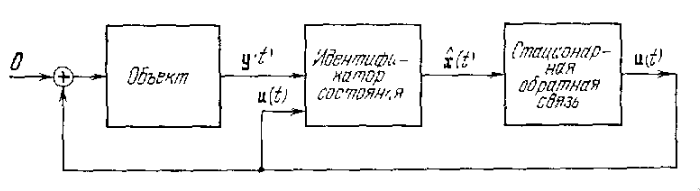
\includegraphics[width=16cm]{Regulator}
\end{center}

\subsection{Применение $n$-мерных идентификаторов}

\begin{theorem}
  Пусть дана полностью управляемая и полностью наблюдаемая система~\eqref{eq:linsys}. Пусть
  матрица $K$ обратной связи $\vb{u}(t) = -K\hat{\vb{x}}(t)$ выбрана так, что характеристический
  полином матрицы $\left[A - BK\right]$ совпадает с заданным многочленом
  $\varphi_{\text{у}}(\lambda) = \lambda^n + \gamma_1 \lambda^{n-1} + \cdots + \gamma_n$,
  и пусть для этой системы построен асимптотический идентификатор состояния полного порядка
  \begin{equation*}
    \dot{\hat{\vb{x}}}(t) = \left[A - LC\right] \hat{\vb{x}}(t) + L \vb{y}(t) + B \vb{u}(t)
  \end{equation*}
  с матрицей $L$ такой, что характеристический полином матрицы $\left[A - LC\right]$
  совпадает с заданным многочленом $\varphi_{\text{и}}(\lambda) = \lambda^n + \beta_1 \lambda^{n-1} + \cdots + \beta_n$.
  Тогда характеристический полином замкнутой системы $2n$-го порядка
  \begin{equation}
    \begin{aligned}
      \dot{\vb{x}}(t) &= A \vb{x}(t) - BK \hat{\vb{x}}(t), \\
      \dot{\hat{\vb{x}}}(t) &= \left[A - LC\right] \hat{\vb{x}}(t)
      + LC \vb{x}(t) - BK \hat{\vb{x}}(t)
    \end{aligned}
  \end{equation}
  совпадает с произведением выбранных полиномов: $\varphi_{\text{з}}(\lambda) = \varphi_{\text{у}}(\lambda) \cdot \varphi_{\text{и}}(\lambda)$.
\end{theorem}

\begin{proof}
  Перепишем замкнутую систему в виде
  \begin{equation*}
    \left[%
    \begin{array}{c}
      \dot{\vb{x}} \\
      \dot{\hat{\vb{x}}}
    \end{array}
    \right]
    =
    \left[
    \begin{array}{cc}
      A & -BK \\
      LC & A - LC - BK
    \end{array}
    \right]
    \left[
    \begin{array}{c}
      \vb{x} \\
      \hat{\vb{x}}
    \end{array}
    \right]
  \end{equation*}

  Сделаем невырожденную замену переменной $\tilde{\vb{x}}(t) = \vb{x}(t) - \hat{\vb{x}}(t)$; матрица
  этого преобразования имеет вид
  \begin{equation*}
    \left[
    \begin{array}{cc}
      E_{n \times n} & 0_{n \times n} \\
      E_{n \times n} & E_{n \times n}
    \end{array}
    \right].
  \end{equation*}
  
  В новых координатах матрица замкнутой системы будет клеточно-диагональной:
  \begin{equation*}
    \left[
    \begin{array}{c}
      \dot{\vb{x}} \\
      \dot{\tilde{\vb{x}}}
    \end{array}
    \right]
    =
    \left[
    \begin{array}{cc}
      A - BK & \ast \\
      0_{n \times n} & A - LC
    \end{array}
    \right]
    \left[
    \begin{array}{c}
      \vb{x} \\
      \tilde{\vb{x}}
    \end{array}
    \right].
  \end{equation*}

  Характеристический полином этой клеточно-диагональной матрицы совпадает с произведением характеристических полиномов
  клеток, стоящих на диагонали, то есть $\varphi_{\text{з}}(\lambda) = \varphi_{\text{у}}(\lambda) \cdot \varphi_{\text{и}}(\lambda)$.
\end{proof}

\subsection{Применение идентификаторов неполного порядка}

Аналогичный результат справедлив и для случая использования идентификатора состояния неполного, 
$(n-p)$--мерного порядка.

Сначала докажем соответствующий результат для системы с одним выходом, когда идентификатор имеет размерность $n-1$.

\begin{theorem}
  Рассмотрим полностью идентифицируемую и полностью управляемую систему с одним выходом:
  \begin{equation*}
    \begin{aligned}
      \dot{\vb{x}}(t) &= A \vb{x}(t) + B \vb{u}(t) \\
      y(t) &= c \vb{x}(t).
    \end{aligned}
  \end{equation*}
  Пусть матрица $K$ обратной связи $\vb{u}(t) = -K\hat{\vb{x}}(t)$ выбрана так, что характеристический полином матрицы $\left[A - BK\right]$
  совпадает с заданным многочленом $\varphi_{\text{у}}(\lambda)$,
  и пусть для этой системы построен $(n-1)$--мерный идентификатор состояния вида
  \begin{equation*}
    \dot{\hat{\vb{x}}}_1(t) = \bar{A} \hat{\vb{x}}_1(t) + \bar{\vb{a}}_n y(t) + B_1 \vb{u}(t), \qquad \hat{\vb{x}}_1(t): \mathbb{R} \to \mathbb{R}^{(n-1)}
  \end{equation*}
  (см.~\cite[с. 282]{Andreev1976}; $B_1$ получена из $B$ заменой элементов последней строки нулями) с заданным многочленом $\varphi_{\text{и}}(\lambda)$.
  Тогда характеристический полином замкнутой системы $(2n-1)$--го порядка
  совпадает с произведением выбранных полиномов: $\varphi_{\text{з}}(\lambda) = \varphi_{\text{у}}(\lambda) \cdot \varphi_{\text{и}}(\lambda)$.
\end{theorem}

\begin{proof}
  Замкнутая система имеет вид
  \begin{equation*}
    \begin{aligned}
      \dot{\vb{x}}(t) &= A \vb{x}(t) - BK \hat{\vb{x}}(t), \\
      \dot{\hat{\vb{x}}}_1(t) &= \overline{A} \hat{\vb{x}}_1(t) + \bar{\vb{a}}_n \hat{x}_n(t) - B_1 K \hat{\vb{x}}(t).
    \end{aligned}
  \end{equation*}
  где
  \begin{equation*}
    \hat{\vb{x}}(t) =
    \left[
      \begin{array}{c}
        \hat{\vb{x}}_1(t) \\
        \hat{x}_n(t)
      \end{array}
      \right], \qquad \hat{\vb{x}}(t): \mathbb{R} \to \mathbb{R}^n.
  \end{equation*}
  Проведём замену переменных $\tilde{\vb{x}}(t) = \hat{\vb{x}}_1(t) - \bar{\vb{x}}(t)$; уравнение замкнутой системы примет вид
  \begin{equation*}
    \left[
    \begin{array}{c}
      \dot{\vb{x}} \\
      \dot{\tilde{\vb{x}}}
    \end{array}
    \right]
    =
    \left[
    \begin{array}{cc}
      A - BK & \ast \\
      0_{(n-1) \times n} & \bar{A}
    \end{array}
    \right]
    \left[
    \begin{array}{c}
      \vb{x} \\
      \tilde{\vb{x}}
    \end{array}
    \right].
  \end{equation*}
  Матрица этой системы клеточно-диагональная, поэтому характеристический многочлен этой системы представим в виде
  $\varphi_{\text{з}}(\lambda) = \varphi_{\text{у}}(\lambda) \cdot \varphi_{\text{и}}(\lambda)$.
\end{proof}

В~\cite[с. 286]{Andreev1976} было показано, что если $\vb{y}(t) : \mathbb{R} \to \mathbb{R}^p$, где $p \neq 0$, то
систему можно представить как прямую сумму подсистем, для каждой из которых выход скалярный, поэтому справедлива
\begin{theorem}
  Пусть линейная система~\eqref{eq:linsys} является полностью управляемой и полностью идентифицируемой и имеет $p$ независимых
  выходов. Тогда можно построить цепь обратной связи $(n-p)$--го порядка такую, что характеристический полином замкнутой системы
  $(2n-p)$--го порядка совпадает с заранее заданным вещественным полиномом $(2n-p)$--го порядка.
\end{theorem}

\section{Заключение}

В работе доказана возможность построения стабилизирующего динамического регулятора для линейной стационарной системы
с идентификаторами как полного, так и пониженного порядка. Полученные результаты в дальнейшем можно обобщить
на системы с запаздыванием и на системы, подверженные помехам и внешним возмущениям.

\newpage

\addcontentsline{toc}{section}{Список использованных источников}
\renewcommand{\refname}{Список использованных источников}
\begin{center}
  \nocite{Kalman2004}
  \nocite{Polyak2019}
  \printbibliography{}
\end{center}

%% \newpage

%% \appendix
%% \addappheadtotoc{}
%% \begin{center}
%%   \textbf{\Large{Приложения}}
%% \end{center}

%% \addcontentsline{toc}{section}{Приложение А. Бла}
%% \renewcommand{\refname}{Приложение А. Бла}

%% \begin{center}
%%   \textbf{\large{Приложение А. Бла}}
%% \end{center}

\end{document}
